% The Methods section should be brief but adequate to allow a qualified investigator to repeat the research. The animals, supplies and equipment used should be described in detail. All companies from which compute resources were obtained should be listed with their location. All methods of analysis and statistical testing must be identified and explained in detail. Studies employing animals have to identify that the experiments being reported were approved by the Institutional Animal Care and Use Committee.
\chapter{Methods}
\label{sec:methods}

We use a family of VLMs called CLIP \citep{clip} for semantic inference and a model-based planning controller using an improved Cross-Entropy Method (iCEM) \citep{icem} as our artificial agent.
This chapter describes the components of our approach, including the mathematical setup, the CLIP model, the intrinsic semantics rewards, and the iCEM controller.

\section{Preliminaries}
\label{sec:preliminaries}
% - Notation
We formulate the problem as a \emph{fully observable} Markov Decision Process (MDP) given by the tuple \((\cS, \cA, \cO, \Theta, \Gamma, R, \bfs_0, \bfo_0)\), with state-space \(\cS \in \nR^{n_s}\), action-space \(\cA \in \nR^{n_a}\), observation-space (image-space) \(\cO \in \nR^{n_o}\), rendering function \(\Theta: \cS \mapsto \cO\), transition kernel (environment model) \(\Gamma: \cS \times \cA \mapsto \cS\), reward function \(R: \cS \times \cO \mapsto \nR\), initial state \(\bfs_0 \in \cS\), and its corresponding initial image observation \(\bfo_0 = \Theta(\bfs_0)\).

A trajectory \(\cT_t = \{(\bfs_t, \bfo_t, r_t, \bfa_t), (\bfs_{t+1}, \bfo_{t+1}, r_{t+1}, \bfa_{t+1}), \ldots \}\) at time \(t\) is a sequence of observation-reward-action tuples starting from the current state \(\bfs_t\), where \(\bfs_k \in \cS\), \(\bfo_k \in \cO\), \(r_k \in \nR\), and \(\bfa_k \in \cA\).
In a typical reinforcement learning (RL) setting, the returns of such a trajectory \(\cT_t\) are the discounted sum of rewards given by,
\begin{equation}
    \label{eq:rl-goal}
    \mathit{\Upsilon}(\cT_t) = \sum_{k=0} \gamma^k r_{t+k},
\end{equation}
where \(r_t\) is the expected reward at time \(t\) and \(\gamma \in [0, 1]\) is the discount factor. The agent's goal is to learn an action policy \(\pi^*: \cS \mapsto \cA\) that maximizes its expected reward;
\begin{equation}
    \label{eq:rl-policy}
    \pi^*_t = \argmax_{\pi} E_{\cT_t \sim \pi} \left[ \mathit{\Upsilon}(\cT_t) \right],
\end{equation}
where the expectation is under trajectories \emph{rolled-out} with \(\bfa_t \sim \pi(\cdot \mid \bfs_t)\), \(\bfs_{t+1} = \Gamma(\bfs_t, \bfa_t)\), \(\bfo_t = \Theta(\bfs_t)\), and \(r_t = R(\bfs_t, \bfo_t)\).

In our formulations, we consider a finite-horizon problem, where the agent is tasked with optimizing the expected return over a limited planning horizon \(\eta\).

\blfootnote{\textbf{Notation}:
We follow the following notation conventions throughout the text, unless explicitly noted otherwise.
Scalars are denoted using lowercase letters, e.g. \(x \in \nR\), and scalar hyperparameters are specially denoted with lowercase Greek letters, eg. \(\chi\).
Vectors are denoted with boldface letters, e.g. \(\bfx \in \nR^n\).
Sets of vectors are denoted italicized boldface letters with a length indicator, e.g. \(\bmx^{(n)} = \{ \bfx_1, \ldots, \bfx_n \}\). The length indicator is omitted for readability at times.
Calligraphic letters are used for higher vector sets, e.g. \(\cX = \{ \bmx^{(n)}_1, \ldots, \bmx^{(n)}_m \}\), and other sets, including spaces (\(\cS, \cA, \cO, \cI, \cL, \cV\)).
Functions are denoted by uppercase letters, e.g. \(\mathrm{X}\), and those with scalar codomains are italicized, eg. \(X\).
This is also true for the reward function denoted by \(R\) whose value is denoted by \(r\). This is not usually the case in RL literature (which denotes them just in the opposite way), but we use this notation to maintain consistency.
However, to avoid radically diverging from the prevalent notations, there are two notable exceptions -- \(\pi\) is used to denote the policy function and \(p\) for probability distributions.
% ``\(r\)'' for denoting reward functions. ``\(R\,\)'' instead denotes a scalar reward value.
}

\newpage    
\section{Vision-Language Models}
\label{sec:vlms}

We define vision-language models (VLMs) as functions capable of processing both language inputs \(\bml \in \cL\) and vision inputs \(\bmi \in \cI\), where \(\cL\) is a set of natural language strings/prompts and \(\cI \subseteq \cO\) is the space of 2D RGB images.

\subsection{CLIP}
\label{sec:clip}
CLIP (Contrastive Language Image Pretraining; \cite{clip}) is a family of vision-language models that have two main components -- an image encoder \(\Psi_I: \cI \mapsto \cV\) and a language encoder \(\Psi_L: \cL \mapsto \cV\), which generate unit magnitude vector embeddings for images and text, respectively, in the same high-dimensional latent space \(\cV \in [0, 1]^{n_v}\), which can thus be compared to each other using a vector similarity metric \(\Lambda: \cI \times \cL \mapsto \nR\), e.g. cosine similarity (\(S_c\), essentially dot product).

For a label \(\bfl \in \cL\) and an image \(\bfi \in \cI\), the similarity is given by,
\begin{equation}
    \label{eq:clip-similarity}
    \Lambda(\bfi, \bfl) := S_c(\Psi_I(\bfi), \Psi_L(\bfl)) = \dfrac{\Psi_I(\bfi) \cdot \Psi_L(\bfl)}{\| \Psi_I(\bfi) \| \| \Psi_L(\bfl) \|} = \Psi_I(\bfi) \cdot \Psi_L(\bfl).
\end{equation}

Eponymously, the CLIP image and text encoders are jointly trained using a contrastive loss which directs the model to semantically align the correct image and text pairs (in the latent space) by increasing their similarity while simultaneously pushing apart the embeddings of the mismatched pairs by decreasing their similarity.

Given a batch of \(n\) image-caption pairs; images \(\bmi^{(n)} = \{ \bfi_1, \dots, \bfi_{n} \}\) and captions \(\bml^{(n)} = \{ \bfl_1, \dots, \bfl_{n} \}\), such that the corresponding entries are paired, CLIP first computes the matrix of cosine similarities, \(\bmLambda^{(n)}(\bmi, \bml) \in \nR^{n \times n}\), where each item \(\bmLambda^{(n)}_{j,k}\) computes the cosine similarity between the image \(\bfi_j\) and caption \(\bfl_k\).
The training batch loss is then computed as the difference between the similarities corresponding to the correct image-caption pairs and the mismatched caption-image pairs, which is then minimized.

There are several variants of CLIP, with different sizes and different architectures for its image encoder (vision transformer \emph{ViT}; \cite{vit}, or residual network \emph{ResNet}; \cite{resnet}).
We used the vision transformer variant (\texttt{ViT-L/14}) for most of our experiments as it gave a good balance of performance and computational efficiency.
It takes image inputs of size \(224 \times 224\) and tokenizes them in patch sizes of \(14 \times 14\) for the vision transformer.
The comparison of the different models from the original paper for our use case is presented in Chapter \ref{sec:clip-comparison} of the appendix.

\subsubsection{CLIP as Zero-Shot Image Classifier}
\label{sec:clip-classifier}
CLIP can be used as a zero-shot classifier by comparing the embeddings of a given image and a set of prompts to predict the likelihood of the image belonging to each of the classes.

Given an image \(\bfi\) and a set of text prompts \(\bml\), the likelihood of the image belonging to the class described by a prompt \(\bfl_k \in \bml\) is given by the softmax function over the similarity scores of the image and the prompt embeddings,
\begin{equation}
    \label{eq:clip-dist}
    P(\bfl_k; \bfi, \bml, \tau) := \dfrac{\exp(\Lambda(\bfi, \bfl_k)/\tau)}{\sum_{\bfl_j \in \bml} \exp(\Lambda(\bfi, \bfl_j)/\tau)},
\end{equation}
where \(\tau \in \nR^+\) is the temperature hyperparameter that controls the flatness of the distribution.
This is an important parameter as it directly controls the quality of our entropy reward \eqref{eq:entropy-reward}.
The original paper suggests a value of \(0.01\) for most purposes, but we usually use values between the range \(0.01 - 0.02\) for our experiments.
See \secref{sec:reg-temperature} for details.

\subsubsection{Prompts for CLIP}
\label{sec:prompt-engineering}
Due to the inherent ambiguity in natural language, the exact phrasing can influence CLIP's inference.
We experiment with this in our investigations.

For objective analysis, we break the structure of a language prompt \(\bfc \in \cL\) representing a creative possibility \(c\) in an environment as ``\(\{\text{prefix}\}\{c\}\{\text{suffix}\}\)'', where ``prefix'' and ``suffix'' are optional context phrases. For example, if \(c =\) ``\texttt{apple}'', then the prompt could be ``\texttt{picture of an apple, on a white background}'', where ``\texttt{picture of an }'' and ``\texttt{, on a white background}'' are the prefix and suffix respectively.

\section{Semantic Rewards for Free Play}
\label{sec:semantics-reward}
This section describes the mathematical formulation of the intrinsic semantic reward that encourages the agent to explore its environment in a semantically expressive manner, akin to free play in humans.
It also gives the necessary background on the additional intrinsic regularity reward that complements it.

\subsection{Semantics Entropy Reward}
\label{sec:entropy-reward}
% - Entropy reward and its regularization hyperparameters derived from the ZEST formulation

Mathematically, in its simplest form, the semantics reward \(R_{\text{semantics-entropy}}: \cO \mapsto \nR\) is formulated as the negative entropy (\(-H\)) of the likelihood of the predictions of the VLM for an image observation \(\bfo \in \cO\) over a set of \(n_c\) creative possibilities \(\bmc = \{ \bfc_1, \bfc_2, \ldots, \bfc_{n_c} \}\);
We call this the \emph{semantics-entropy reward},
\begin{equation}
    \label{eq:entropy-reward}
    R_{\text{semantics-entropy}}(\bfo; \bmc, \tau) := -H(p(\bmc \mid \bfo; \tau)) = \sum_{\bfc_k \in \bmc} P(\bfc_k \mid \bfo; \bmc, \tau) \log P(\bfc_k \mid \bfo; \bmc, \tau).
\end{equation}
% 
\subsubsection{Goal-Baseline Regularization}
\label{sec:goal-baseline}
To improve the reward quality (shape), we further extend this formulation by adopting a combination of suggestions from other studies on VLMs as a source of goal-conditioned rewards.

The most trivial way to use CLIP as a goal-conditioned reward is to directly use the similarity metric from \eqref{eq:clip-similarity} as the reward function.
Given a goal description \(\bfg \in \cL\), the reward for an image observation \(\bfo \in \cO\) is given by,
\begin{equation}
    \label{eq:trivial-reward}
    R_{\text{clip}}(\bfo; \bfg) := S_c(\Psi_I(\bfo), \Psi_L(\bfg)).
\end{equation}
This captures the projection of the image observation embedding \(\bfo\) onto the direction spanned by the goal embedding \(\bfg\).

\cite{zest} developed an alternative method called \emph{ZeST} (zero-shot task specification) which employs \emph{delta embeddings} that use the difference in embeddings between the desired and initial/\emph{baseline} configurations, for both image and text inputs, to directionally remove irrelevant parts of the CLIP representation.
The goal-baseline regularized reward function in this case is the similarity between the delta embeddings,
\begin{equation}
    \label{eq:zest}
    R_{\text{zest}}(\bfo; \bfo_b, \bfg, \bfg_b) := S_c((\Psi_I(\bfo) - \Psi_I(\bfo_b)), (\Psi_L(\bfg) - \Psi_L(\bfg_b))).
\end{equation}
where \(\bfg_b \in \cL\) is a natural language description of the initial/baseline environment image observation \(\bfo_b = \bfo_0\).

Intuitively, providing a baseline sets the context of the setup, and the direction from a baseline \(\bfg_b\) to goal \(\bfg\) captures the desired change from the environment's image baseline \(\bfo_b\) to the target state.
As an example, consider the case where the goal is to draw a circle starting from a blank canvas i.e. the goal \(\bfg\) is something like ``a circle on a white background''.
Then the baseline \(\bfg_b\) could be ``a blank canvas'' and the image observation baseline \(\bfo_b\) would be the starting blank canvas image.

\cite{negprompt} further proposed a negative prompt formulation that used the negations of goal states, instead of descriptions of the initial states, as goal baselines.
In the example, this would be ``not a circle on a white background''.

These delta embeddings considerably improve performance in language-guided goal-conditioned tasks by providing a more focused reward signal.
However, it is not certain that the direction from the baseline to the goal captures all the relevant information.
Therefore, instead of using one or the other, \cite{vlmrm} further made a trade-off between the two projections in their \emph{VLM-RM} method and proposed a goal-baseline regularization technique that considered both -- the similarity of the image observation to the target and also the direction from the baseline towards the goal in the CLIP embedding space.

VLM-RM does not use delta embeddings or baselines for the image input, but only for the text input.
Their formulation is given by,
\begin{equation}
    \label{eq:vlmrm}
    R_{\text{goal-reg}}(\bfo; \bfg, \bfg_b, \gamma) := 1 - \dfrac{1}{2}\ \norm{\gamma\ \text{proj}_{\bfv}\Psi_I(\bfo) + (1 - \gamma)\ \Psi_I(\bfo) - \Psi_L(\bfg)}^2_2,
\end{equation}
where \[\bfv := \frac{\Psi_I(\bfg) - \Psi_L(\bfg_b)}{\norm{\Psi_I(\bfg) - \Psi_L(\bfg_b)}}\] is the direction spanned by the vector between the embeddings of \(\bfg\) and \(\bfg_b\), \[\text{proj}_{\bfv}\Psi_I(\bfo) := (\bfo \cdot \bfv)\,\bfv\] is the projection of the image observation embedding \(\bfo\) onto this direction, and \(\gamma \in [0, 1]\) is a hyperparameter to control the trade-off/regularization strength\footnote{We want to note here that the official implementation of VLM-RM available at \url{https://github.com/AlignmentResearch/vlmrm} is slightly different from the formulation given in the original paper, which is used here. Simplifying the other formulation leads to an additional term in the reduced form, but the overall essence of the reward from a conceptual standpoint still holds.}.
% 
% \begingroup
% \allowdisplaybreaks
\vspace{-1.5pt}
\begin{align}
    % R_{\text{goal-reg}}(\bfo; \bfg, \bfg_b, \gamma) &= 1 - \dfrac{1}{2}\ \norm{\gamma\ \text{proj}_{\bfv}\Psi_I(\bfo) + (1 - \gamma)\ \Psi_I(\bfo) - \Psi_L(\bfg)}^2_2, \label{eq:vlmrm}
    % \intertext{where \(\bfv\) is the direction spanned by \(\Psi_I(\bfg_b) - \Psi_L(\bfg)\), \(\text{proj}_{\bfv}\Psi_I(\bfo)\) is the projection of the image observation embedding \(\bfo\) onto this direction, and \(\gamma \in [0, 1]\) is a hyperparameter to control the regularization/trade-off strength.
    % Note that the magnitude of the projection \(\norm{\text{proj}_{\bfv}\Psi_I(\bfo)}_2\) is equivalent to the cosine similarity \(\cos(\vartheta) := S_c(\Psi_I(\bfo), (\Psi_L(\bfg) - \Psi_L(\bfg_b)))\), and \(\sin(\vartheta)\) is the projection of \(\bfo\) perpendicular to this direction.
    % The authors found this method to be relatively robust to changes in \(\gamma\) with most intermediate values being better than \(0\) or \(1\).}
    \shortintertext{For \(\gamma = 0\), the original CLIP similarity metric from \eqref{eq:clip-similarity} is recovered as an unregularized goal-conditioned reward function after simplification (since all embeddings are unit vectors, i.e. \(\norm{\Psi(\cdot)}_2 = 1\));}
    R_{\text{goal-reg}}(\bfo; \bfg, \bfg_b, 0) &= 1 - \dfrac{1}{2}\ \norm{\Psi_I(\bfo) - \Psi_L(\bfg)}^2_2 = S_c(\Psi_I(\bfo), \Psi_L(\bfg)). \label{eq:vlmrm-0}
    \intertext{For \(\gamma = 1\), there is a trade-off of components of \(\bfo\) orthogonal and parallel to ``\(\bfg - \bfg_b\)''.
    % Thus, it only retains the components that align with the direction from the baseline to the goal.
    % \texttt{-- A claim from the original paper; is incorrect!}
    }
    R_{\text{goal-reg}}(\bfo; \bfg, \bfg_b, 1) &= 1 - \dfrac{1}{2}\ \norm{\text{proj}_{\bfv}\Psi_I(\bfo) - \Psi_L(\bfg)}^2_2\\
    &= 1 - \dfrac{\norm{\text{proj}_{\bfv}\Psi_I(\bfo)}^2_2 + 1 - 2\ \text{proj}_{\bfv}\Psi_I(\bfo) \cdot \Psi_L(\bfg)}{2}\\
    &= \underbrace{\dfrac{1 - \norm{\text{proj}_{\bfv}\Psi_I(\bfo)}^2_2}{2}}_{\propto\ \sin^2(\vartheta)} + \underbrace{\dfrac{\Psi_I(\bfo) \cdot (\Psi_L(\bfg) - \Psi_L(\bfg_b))}{2}}_{\propto\ \cos(\vartheta)}. \label{eq:vlmrm-1}
\end{align}
% (Refer to equations \eqref{eq:vlmrm-equivalence-start} to \eqref{eq:vlmrm-equivalence-end} for more details on the derivation.)\\
% Mathematically, this is not equivalent to \eqref{eq:zest} (with no image baseline), because of the additional term, but it is similar in spirit.
% \endgroup

Note that the magnitude of the projection \(\norm{\text{proj}_{\bfv}\Psi_I(\bfo)}_2\) is equal to the cosine similarity \(\cos(\vartheta) := S_c(\Psi_I(\bfo), (\Psi_L(\bfg) - \Psi_L(\bfg_b)))\), and \(\sin(\vartheta)\) is the projection of \(\Psi_I(\bfo)\) perpendicular to this direction.

The authors found this method to be relatively robust to changes in \(\gamma\) with most intermediate values being better than \(0\) or \(1\).

\newpage
\subsection{Regularized Semantics Entropy Reward}
\label{sec:entropy-reward-reg}
We combine these ideas below to derive a \emph{baseline regularized semantics-entropy reward} from \eqref{eq:entropy-reward}.\\
Let \(\bmp := \text{proj}_{\bfv}\Psi_I(\bfo)\), \(\bmo := \Psi_I(\bfo),\ \bmg := \Psi_L(\bfg),\ \bmg_b := \Psi_L(\bfg_b)\) for brevity, then using the property \(\norm{\bmo}_2 = \norm{\bmg}_2 = \norm{\bmg_b}_2 = 1\) and the results \(\bmp \cdot \bmo = \norm{p}^2_2\) and \(\bmp \cdot \bmg = (\bmg - \bmg_b) \cdot \bmo\ /\ 2\), the VLM-RM reward can be simplified as,
\vspace{-1.5pt}
\begin{align}
    &1 - \dfrac{1}{2} \norm{\gamma\ \bmp + \left(1 - \gamma\right) \bmo - \bmg}^2_2 \tag{\(R_{\text{goal-reg}}\), from \ref{eq:vlmrm}}\\
    \label{eq:vlmrm-equivalence-start}
    &= 1 - \dfrac{1}{2} \Big[\norm{\gamma\ \bmp + \left(1 - \gamma\right) \bmo}^2_2 + \cancelto{1}{\norm{\bmg}^2_2} &&- 2 \left(\gamma\ \bmp + \left(1 - \gamma\right) \bmo\right) \cdot \bmg\Big]\\
    &= \dfrac{1 - \norm{\gamma\ \bmp + \left(1 - \gamma\right) \bmo}^2_2}{2} &&+ \gamma\ \bmp \cdot \bmg + \left(1 - \gamma\right) \bmo \cdot \bmg\\
    &= \dfrac{1 - \norm{\gamma \left(\bmp - \bmo\right) + \bmo}^2_2}{2} &&+ \dfrac{\gamma}{2} \left(\bmg - \bmg_b\right) \cdot \bmo + \left(1 - \gamma\right) \bmg \cdot \bmo\\
    &= \dfrac{1 - \gamma^2\ \norm{\bmp - \bmo}^2_2 - 2 \gamma \left(\bmp - \bmo\right) \cdot \bmo - \cancelto{1}{\norm{\bmo}^2_2}}{2} &&+ \left(\dfrac{\gamma}{2} \left(\bmg - \bmg_b\right) + \left(1 - \gamma\right) \bmg\right) \cdot \bmo\\
    &= \dfrac{-\gamma^2 \left(\norm{\bmp}^2_2 + \norm{\bmo}^2_2 - 2\ \bmp \cdot \bmo\right) - 2 \gamma \left(\bmp \cdot \bmo - \norm{\bmo}^2_2\right)}{2} &&+ \left(\dfrac{\gamma}{2}\ \bmg - \dfrac{\gamma}{2}\ \bmg_b + \bmg - \gamma\ \bmg\right) \cdot \bmo\\
    % &= \dfrac{-\gamma^2 \big(\norm{\bmp}^2_2 + \cancelto{1}{\norm{\bmo}^2_2} - 2\ \bmp \cdot \bmo\big) - 2 \gamma \big(\bmp \cdot \bmo - \cancelto{1}{\norm{\bmo}^2_2}\big)}{2} &&+ \left(\dfrac{\gamma}{2}\ \bmg - \dfrac{\gamma}{2}\ \bmg_b + \bmg - \gamma\ \bmg\right) \cdot \bmo\\ % above with cancellations
    &= \dfrac{-\gamma^2 \left(\norm{\bmp}^2_2 + 1 - 2\ \norm{\bmp}^2_2\right) - 2 \gamma \left(\norm{\bmp}^2_2 - 1\right)}{2} &&+ \left(\bmg - \dfrac{\gamma}{2}\ \bmg - \dfrac{\gamma}{2}\ \bmg_b\right) \cdot \bmo\\
    &= \dfrac{-\gamma^2 + 2\gamma}{2} + \dfrac{\gamma^2\ \norm{\bmp}^2_2 - 2 \gamma\ \norm{\bmp}^2_2}{2} &&+ \left(\left(1 - \dfrac{\gamma}{2}\right) \bmg - \dfrac{\gamma}{2}\ \bmg_b\right) \cdot \bmo\\ % additional step
    %% Option 1 -- p^2 term
    &= \gamma\left(1 - \dfrac{\gamma}{2}\right)\left(1 -\norm{\bmp}^2_2\right) &&+ \left(\left(1 - \dfrac{\gamma}{2}\right) \bmg - \dfrac{\gamma}{2}\ \bmg_b\right) \cdot \bmo\\
    &= \underbrace{\gamma\left(1 - \dfrac{\gamma}{2}\right)\left(\sin\left(\vartheta\right)\right)}_{\text{Term \#1 (\(\perp\))}} &&+ \underbrace{\left(\left(1 - \dfrac{\gamma}{2}\right) \bmg - \dfrac{\gamma}{2}\ \bmg_b\right) \cdot \bmo}_{\text{Term \#2 (\(\parallel\))}}.
    %% Option 2 -- constant term separated
    % &= \gamma\left(1 - \dfrac{\gamma}{2}\right) -\ \gamma \left(1 - \dfrac{\gamma}{2}\right)\norm{\bmp}^2_2 &&+ \left(\left(1 - \dfrac{\gamma}{2}\right) \bmg - \dfrac{\gamma}{2}\ \bmg_b\right) \cdot \bmo\\
    % &= \underbrace{\gamma\left(1 - \dfrac{\gamma}{2}\right)}_{\textstyle\text{constant}} -\ \underbrace{\gamma \left(1 - \dfrac{\gamma}{2}\right)\left(\bmo \cdot \dfrac{\left(\bmg - \bmg_b\right)}{\norm{\bmg - \bmg_b}_2}\right)^2}_{\text{Term \#1 (\(\perp\))}} &&+ \underbrace{\left(\left(1 - \dfrac{\gamma}{2}\right) \bmg - \dfrac{\gamma}{2}\ \bmg_b\right) \cdot \bmo}_{\text{Term \#2 (\(\parallel\))}}.
    \label{eq:vlmrm-equivalence-end}
\end{align}
Term \#1 captures the projection perpendicular to the direction from the baseline to the goal and Term \#2 captures the trade-off of projection along this direction and the goal.
To simplify further, we consider only the latter in our formulation as it contains the desired information about the goal.
We adopt this term as the basis to add baseline regularization to the semantics-entropy reward in \eqref{eq:entropy-reward-reg} and consider similar delta embeddings for the image observation space as well.

First, let us formulate a regularized similarity metric for an image observation \(\bfi \in \cI\) with baseline image \(\bfi_b \in \cI\) and target label \(\bfl \in \cL\) with baseline \(\bfl_b \in \cL\);
\begin{equation}
    \label{eq:clip-similarity-reg}
    \begin{split}
        \hat{\Lambda}(\bfi, \bfl; \bfi_b, \bfl_b, \alpha_{l}, \beta_{i})
        &:= S_c(
            ((1 - \beta_{i})\ \Psi_I(\bfi) - \beta_{i}\ \Psi_I(\bfi_b)),
            ((1 - \alpha_{l})\ \Psi_L(\bfl) - \alpha_{l}\ \Psi_L(\bfl_b))
        ),
    \end{split}
\end{equation}
where \(\alpha_{l}, \beta_{i} \in [0, 0.5]\) are the regularization hyperparameters homologous to \(\gamma / 2\) in \eqref{eq:vlmrm-equivalence-end}, for text and image inputs respectively, and \(\tau \in \nR^+\) is the temperature hyperparameter.

The updated likelihood distribution \(\hat{p}\) of the predictions of the VLM for the image observation \(\bfo \in \cO\) over the creative possibilities \(\bmc \subset \cC\) using this regularized similarity metric is then given by,
\begin{equation}
    \label{eq:clip-dist-reg}
    \hat{P}(\bfc_k \mid \bfo; \bfo_b, \bmc, \bfc_b, \alpha_{l}, \beta_{i}, \tau) := \dfrac{\exp(\hat{\Lambda}(\bfo, \bfc_k; \bfo_b, \bfc_b, \alpha_{l}, \beta_{i})/\tau)}{\sum_{\bfc_j \in \bmc} \exp(\hat{\Lambda}(\bfo, \bfc_k; \bfo_b, \bfc_b, \alpha_{l}, \beta_{i})/\tau)},
\end{equation}
where \(\bfc_k \in \bmc\). Using these definitions, the regularized semantics-entropy reward is given as,
\begin{align}
    R_{\text{sem-entropy-reg}}(\bfo; \bfo_b, \bmc, \bfc_b, \alpha_{l}, \beta_{i}, \tau)
    &:= -H(\hat{p}(\bmc \mid \bfo; \bfo_b, \bfc_b, \alpha_{l}, \beta_{i}, \tau)) \label{eq:entropy-reward-reg}\\
    &\ = \sum_{\bfc_k \in \bmc} \hat{P}(\bfc_k \mid \bfo; \bfo_b, \bmc, \bfc_b, \alpha_{l}, \beta_{i}, \tau) \log \hat{P}(\bfc_k \mid \bfo; \bfo_b, \bmc, \bfc_b, \alpha_{l}, \beta_{i}, \tau), \nonumber
\end{align}
where \(\bfc_b\) is the text baseline, which could either be the initial state description or the negation of the goal.

\newpage
\subsection{Regularity Reward}
\label{sec:regularity-reward}
We complement the semantic reward with regularity as an intrinsic reward (\emph{RaIR}) \citep{rair}, which encourages the agent to create regular and symmetric patterns in its creations.
The authors described the regularity reward RaIR as ``(the) redundancy in the description of the situation, to measure the degree of sub-structure recurrence''.

Mathematically, we consider that the state space can be factorized into a composition of the different (\(n_e\)) entities in the environment and the configuration of the agent, \(\cS = (\cS_{\text{obj}})^{n_e} \times \cS_{\text{agent}}\), where \(\cS_{\text{obj}} \in \nR^d\); \(d = 2\) in our environments. %, such that \(n_s = n_e \cdot d\).
This allows the RaIR reward \(R_{\text{RaIR}}: \cS \mapsto \nR\) to be formulated in terms of multiplicities \(M: \cX \mapsto \nN\) (counts of occurrence) of the sub-structures \(\cX\) in the arrangement of the different entities of the environment in the state \(\bfs\),
\begin{equation}
    \label{eq:rair}
    R_{\text{RaIR}}(\bfs; \omega) := -H(\mathrm{\Omega}(\bfs; \omega)) = \sum_{\cX \in \mathrm{\Omega}(\bfs)} P(\cX; \omega) \log P(\cX; \omega),
\end{equation}
where \(\mathrm{\Omega}\) is a factorization function that decomposes a state \(\bfs\) into a multiset of its unique sub-structures given the hyperparameters \(\omega\) (resolution, bidirectionality),
\begin{equation}
    \label{eq:rair-factorization}
    \mathrm{\Omega} : (\cS_{obj})^{n_e} \mapsto \{ \cX_1^{M(\cX_1)}, \cX_2^{M(\cX_2)}, \ldots \},
\end{equation}
and \(P(\cX; \omega)\) is the probability of a sub-structure \(\cX \in \mathrm{\Omega}(\bfs; \omega)\) in the state \(\bfs\) calculated as,
\begin{equation}
    \label{eq:rair-probability}
    P(\cX; \omega) = \dfrac{M(\cX)}{\sum_{\cX' \in \mathrm{\Omega}(\bfs; \omega)} M(\cX')}.
\end{equation}
% 
For our purposes, following insights from \cite{symmetry} and \cite{compositional}, we use the relational formulation of RaIR which captures the pairwise relationships between the entities of the environment in the state \(\bfs\) by calculating the distances between them in the discretized coordinate space;
\begin{equation}
    \label{eq:rair-relational}
    \mathrm{\Omega}(\bfs) = \{ \cX^{M(\cX)} : \cX = \lfloor s^{(j)} - s^{(k)} \rceil \mid s^{(j)}, s^{(k)} \in \bfs \},
\end{equation}
where the \(\lfloor \cdot \rceil\) operator groups the distances into discrete bins based on the configured resolution.
For more details on the parameters and formulation, please refer to \secref{sec:regularity-reward-details} of the appendix.

\subsection{Complete Intrinsic Semantics Reward}
\label{sec:complete-semantics-reward}
The complete intrinsic semantics reward \(R_{\text{semantics}}\) is then given as the weighted sum of the regularity reward \(R_{\text{RaIR}}\) and the regularized semantics-entropy reward \(R_{\text{semantics-entropy-reg}}\);
\begin{equation}
    \label{eq:semantics-reward}
    R_{\text{semantics}}(\bfs, \bfo; \bfo_b, \bmc, \bfc_b, \alpha_{l}, \beta_{i}, \tau) =R_{\text{semantics-entropy-reg}}(\bfo; \bfo_b, \bmc, \bfc_b, \alpha_{l}, \beta_{i}, \tau) + \lambda\ R_{\text{RaIR}}(\bfs),
\end{equation}
where \(\lambda\) is a hyperparameter that controls the trade-off between the two rewards.

To be able to properly compare the two rewards, we constrain them to the same range \([0, 1]\) by normalizing them with their maximum possible entropy.
The regularity reward is normalized by the maximum possible entropy of the multiset -- \(\log\left(\binom{n_e}{2}\right)\), which is equal to the entropy of a uniform distribution over the \(\binom{n_e}{2}\) possible pairwise object distances of the \(n_e\) entities/objects in the state space, and
the semantics-entropy reward is normalized by the maximum possible entropy of the likelihood distribution over the creative possibilities, which is \(\log(n_c)\), where \(n_c\) is the number of creative possibilities.

\newpage
\section{iCEM}
\label{sec:icem}
% The Cross-Entropy Method (CEM) is an adaptive importance sampling procedure.

In the Model-Based Reinforcement Learning (MBRL) paradigm, the agent learns a model \(\Gamma\) of the MDP dynamics from interactions with the environment and uses it to predict the consequences of its actions which enables it to plan for the best policies.
Such policies can be learned with universal function approximators such as neural networks using RL algorithms or planning methods.

The improved Cross-Entropy Method (iCEM) is one such planning method.
It is a zeroth-order Monte-Carlo trajectory optimizer that works in a Model Predictive Control (MPC) loop to solve finite-horizon planning problems online, i.e. it iteratively re-plans after every step in the environment by (1) coming up with several action sequences (by sampling a multi-variate distribution) to \emph{think} a few steps ahead, (2) imagining/predicting the future states resulting from these actions (using the model of the environment) and assessing their expected returns (using the reward function), (3) picking out the best action sequences, (4) improving the \emph{thinking} method based on these elite sequences, and (5) taking the first step of the best action sequence.

Precisely, given a finite planning horizon \(\eta\), iCEM uses a clipped colored-noise Gaussian distribution of dimension \(n_a \times \eta\) over action sequences (\(\bma^{(\eta)} = \{ \bfa_0, \bfa_1, \ldots, \bfa_{\eta-1} \}\)), given by,
\begin{equation}
    \label{eq:icem-distribution}
    p(\bma^{(\eta)}) = \text{clip}(\bmmu_t + \cC^\beta(n_a, \eta) \odot \bmsigma_t^2),
\end{equation}
where \(\bmmu_{t}, \bmsigma_{t} \in \nR^{n_a \times \eta}\) are the mean and standard deviation of the sampling distribution at time \(t\) respectively, and \(\cC^\beta(n_a, \eta)\) is a sampling function that returns \(n_a\) (one for each action dimension) sequences of length \(\eta\) sampled from colored noise normal distribution with exponent \(\beta\) (\(= 1\) in our experiments; pink noise), zero mean, and unit variance.

At every timestep \(t\), there are multiple \emph{inner} iterations of the following calculations.
At inner iteration \(i\),\\
(1) starting with a sampling distribution \( p(\bmmu_{t}^{i - 1},\bmsigma_{t}^{i - 1})\), a fixed-length (\(\nu\)) set of action sequences (\(\cA_t = \{ \bma^{(\eta)}_1, \bma^{(\eta)}_2, \ldots, \bma^{(\eta)}_{\nu} \}\)) is sampled from this distribution.
These samples are augmented with a fraction \(\zeta\) of the best action sequences (called the \emph{elite-set} \(\cE_t^{i - 1}\)) from the previous inner iteration (called \emph{keep-elites}) or the previous timestep (called \emph{shift-elites}) if \(i = 0\); this is denoted by \(\zeta \cdot \cE_t^{i - 1}\) in \eqref{eq:icem-augment}. 
Additionally, to ensure that the mean action of the distribution is accessible to the controller, in the last inner iteration \(\iota\), the mean of the distribution \(\bmmu_t\) is added to the elite-set \(\cA^+\);
\begin{equation}
    \label{eq:icem-augment}
    \cA^+_t = \cA_t \cup \begin{cases}
            \zeta \cdot \cE_{t - 1}^\iota & \text{if } i = 0,\\
            \zeta \cdot \cE_t^{\iota - 1} \cup \{ \bmmu_t^\iota \} & \text{if } i = \iota,\\
            \zeta \cdot \cE_t^{i - 1} & \text{otherwise}.
    \end{cases}
\end{equation}

(2) Every action sequence in this augmented set \(\cA^+_t\) is then rolled out (\emph{in imagination}) using the environment model \(\Gamma\) and rendering function \(\Theta\) from the current state \(\bfs_t\) to predict their corresponding expected states and image observations respectively,
\vspace{-1.5pt}
\begin{align}
    \cS_t &= \{ \{ \bfs_{t+1}, \bfs_{t+2}, \ldots, \bfs_{t+\eta} \} \}_{j=1}^{\nu}, \label{eq:icem-rollout}\\
    \cO_t &= \{ \{ \bfo_{t+1}, \bfo_{t+2}, \ldots, \bfo_{t+\eta} \} \}_{j=1}^{\nu}, \label{eq:icem-observations}
    \intertext{where \(\bfs_t = \Gamma(\bfs_{t-1}, \bfa_{t-1})\) and \(\bfo_t = \Theta(\bfs_t)\). The predicted states are evaluated according to the reward function \(r\) to get their corresponding rewards,}
    \cR_t &= \{ \{ r_{t+1}, r_{t+2}, \ldots, r_{t+\eta} \} \}_{j=1}^{\nu}, \label{eq:icem-rewards}
\end{align}
where \(r_{t} = R(\bfs_t, \bfo_t) = \sum_k \lambda_k r_k(\bfs_t, \bfo_t)\) is the weighted sum of all the intrinsic rewards.
The corresponding trajectories are,
\begin{equation}
    \label{eq:icem-trajectories}
    \cT^{(\nu \times \eta)}_t = \{\{(\bfs_t, \bfo_t, r_t, \bfa_t), \ldots, (\bfs_{t+\eta-1}, \bfo_{t+\eta-1}, r_{t+\eta-1}, \bfa_{t+\eta-1}), (\bfs_{t+\eta}, \bfo_{t+\eta}, r_{t+\eta}, \varnothing) \}\}_{j=1}^{\nu}.
\end{equation}
% 
(3) Subsequently, a new elite-set of actions \(\cE_t^i\) of given size \(\kappa\) is determined; it consists of the best \(\kappa\) action sequence samples that maximize an aggregation of the returns from their expected states according to a reward aggregation function \(\mathit{\Upsilon}\);
\begin{equation}
    \label{eq:icem-filter}
    \cE_t^i = \kappa \cdot \cA^+_t = \underset{\text{Best \(\kappa\) action sequences in the augmented set of samples \(\cA^+_t\)}}{\{ \bma^{(\eta)}_k \in \cA^+_t :\ \mid \bma^{(\eta)}_j \in \cA^+_t : \mathit{\Upsilon}(\cT^{(\eta)}_k) \leq \mathit{\Upsilon}(\cT^{(\eta)}_j) \mid\ \leq \kappa \}}.
\end{equation}
More information about the reward aggregation strategies used in our experiments is provided in \autoref{sec:reward-aggregation}.

(4) These new elite action sequences are finally used to refine the distribution to maximize the expected return of its samples.
\vspace{-1.5pt}
\begin{align}
    \label{eq:icem-update}
    \bmmu_{t}^i &= \alpha\ \bmmu_t^{i - 1} + (1-\alpha)\bmmu^{\cE_t^i},\\
    (\bmsigma_{t}^i)^2 &= \alpha(\bmsigma_t^{i - 1})^2 + (1-\alpha)(\bmsigma^{\cE_t^i})^2,
\end{align}
where \(\alpha \in [0, 1]\) is a \emph{momentum} factor.

The above steps are repeated for \(\iota\) inner iterations at every timestep.
At the end of this process, the distribution concentrates on action sequences with high returns, and the best action sequence converges to an optimum;
\begin{equation}
    \label{eq:planning-goal}
    \bma^{(\eta)*} = \argmax_{\bma^{(\eta)}_k \in \cA^+} \mathit{\Upsilon}(\cT^{(\eta)}_k).
\end{equation}
(5) Finally, the first action of the best elite sequence of actions \(\bma^{(\eta)*}_t\) is executed in the environment.
The process is repeated for a specified number of rollout steps or until a terminal state or reward threshold is reached.

% There are additional features that the original iCEM implementation provides, such as decaying population size over time. 
Since the standard deviation in iCEM adapts according to the elite-set statistics, when the controller is close to an optimum, the standard deviation automatically decreases, narrowing down the search and fine-tuning the solution.
Therefore it is sufficient to sample fewer action sequences as the CEM iterations proceed.
Thus, the population size is exponentially decayed over time with factor \(\delta\). 
At timestep \(t\), it is equal to \(max(\nu \delta^{-t}, 2\kappa)\), where the max ensures that the population size is at least double the size of the elite-set.

Since iCEM is a zero-order trajectory optimizer with a limited sample budget and finite-horizon planning, we do not necessarily converge to the global optima.
Although this does not solve the full reinforcement learning problem (infinite horizon and stochastic environments), it is very powerful in optimizing for tasks ad-lib without further adaptation, which makes it suitable for optimizing changing exploration targets in sparse reward scenarios, as in our case (because of noisy CLIP rewards; discussed later in \secref{sec:inference-noise}).

The colored noise of the iCEM distribution leads to temporally correlated action sequences over the horizon for smoother trajectories, which helps mitigate the problems due to the noisy nature of our semantics entropy reward by effectively regularizing the reward landscape.
Furthermore, the addition of memory gives it good sample efficiency, which is essential for our case due to the computational bottleneck because of the long inference times for CLIP.
These reasons made iCEM a suitable choice for our experiments.

For this to be successful, a good transition model \(\Gamma\) needs to be learned, and the reward function needs to be known or discovered.
In our case, the reward function is well-defined, and to evaluate the efficacy of our entropy minimization objective in achieving good semantic expression,
we run simulations using ground truth (GT) models, i.e. with access to the true simulator of the environment itself.
Thus, we can perform multi-horizon planning without accumulating any model errors, which allows us to better investigate the shape and global/local optima of our semantics reward landscape. 

\subsection{Reward Aggregation Strategies}
\label{sec:reward-aggregation}
There are many different ways to aggregate the rewards of the trajectory samples over the horizon.
This is treated as one of the hyperparameters in our experiments.
\vspace{-13.5pt}
\begin{align}
\intertext{A trivial reward aggregation function is the sum of the rewards over the horizon (\texttt{sum}),}
\texttt{sum}(\cT^{(\eta)}) &= \sum_{k=1}^{\eta} r_k. \label{eq:reward-aggregation-sum}
\intertext{We further experimented with a discount factor \(\gamma \in \nR^+\) over the horizon, but usually set it to \(1.0\);}
\texttt{sum-\emph{\(\gamma\)}}(\cT^{(\eta)}) &= \sum_{k=1}^{\eta} \gamma^{k-1} r_k. \label{eq:reward-aggregation-sum-discount}
\intertext{However, this type of consolidating aggregation strategy is not suitable for cases where an increase in return can be preceded by an initial decrease (as a consequence of leaving local optima). So we also considered the \texttt{best} method, which uses the best return over the planning horizon;}
\texttt{best}(\cT^{(\eta)}) &= \max_{k=1}^{\eta} r_k. \label{eq:reward-aggregation-best}
\intertext{Additionally, to combine the better qualities of both the \texttt{sum} and \texttt{best} methods; we formulated a dynamic reward aggregation method that ranks trajectories based on the highest sum of consecutive rewards in a window of a predefined hyperparamterized length \(l\), \texttt{best-\emph{l}};}
\texttt{best-\emph{l}}(\cT^{(\eta)}) &= \max_{k=1}^{\eta-l+1} \sum_{j=k}^{k+l-1} r_{k+j}. \label{eq:reward-aggregation-best-dynamic}
\intertext{Another strategy is to assess the trajectories based on their last states (\texttt{last}), i.e. to simply consider only what the agent could potentially achieve at the end of the horizon.
This is particularly useful when inferring the reward is expensive, as in our case, because only one final state needs to be evaluated;}
\texttt{last}(\cT^{(\eta)}) &= r_h. \label{eq:reward-aggregation-last}
\intertext{Finally, we also experimented with a combination of the \texttt{sum} and \texttt{last} methods with \texttt{last-\emph{l}}, which is the sum of the returns of the last \(l\) steps of the trajectory;}
\texttt{last-\emph{l}}(\cT^{(\eta)}) &= \sum_{k=\eta-l+1}^{\eta} r_k. \label{eq:reward-aggregation-sum-last}
\end{align}

Note that we often use the term \emph{cost} (\(-1 \times r\)) instead of reward in our results and discussions. This is because the iCEM controller implementation we use minimizes costs instead of maximizing rewards, which are essentially equivalent and only differ in their signs.

\section{Experiment Setup}
\label{sec:experiment-setup}

The simulations are run concurrently on multiple NVIDIA V100 and A100 GPUs, depending on the size of the simulations, which is determined by the size of the CLIP model used, the number of trajectory samples in iCEM, and the number of planning horizons.
To minimize the time of a rollout, all \(\eta \times \nu\) CLIP inferences for planning at an inner iCEM iteration are performed in a single batch in parallel.
Environment rendering and simulations are multi-processed on CPU in parallel.

Several optimizations were put into place to improve the simulation time, particularly in environment rendering and CLIP preprocessing.
Please refer to Chapter \ref{sec:efficiency} of the appendix for more details.

\section{Environments}
\label{sec:environments}
We use two custom environments in our experiments which allow for rich creative expression.

\begin{figure}[H]
    \centering
    \subfloat[\centering ShapeGridWorld]{\fbox{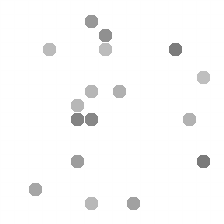
\includegraphics[width=0.4\textwidth]{images/sgw_random.png}}}
    \qquad
    \subfloat[\centering Tangram]{\fbox{
\includegraphics[width=0.4\textwidth]{images/tangram_random.png}}}
    \caption{The environments.}
    \label{fig:environments}
\end{figure}

\subsection{ShapeGridWorld}
\label{sec:sgw}
ShapeGridWorld (SGW) is a pixel grid environment where the agent can draw on the grid by moving pixels around, either one or all of them at the same time.
This is reminiscent of the pin-board platform used in the free play study conducted by \citet{diggs} (\figref{fig:diggs}).
By setting the pixels in a specific layout, the agent can draw a variety of shapes on the grid.
This environment is adapted from the pixel grid environment used in the work by \citet{rair} with some modifications summarised in \ref{sec:sgw-details} of the appendix.

ShapeGridWorld was mostly used in the initial experiments but it eventually proved to promote noise in CLIP inferences which led to underwhelming results.
To work around the problems, the Tangram environment was developed.

\subsection{Tangram}
\label{sec:tangram}
Tangram is a traditional puzzle game consisting of a canvas and seven geometric shapes -- five right isosceles triangles (two large, one medium, and two small), one square, and one parallelogram, which conventionally have distinct colors.
These shapes can be rotated, flipped, and translated on the canvas, without overlapping.
Even though this is a very simple setup, these pieces can be arranged in very different configurations to create expressive abstract patterns.

The Tangram virtual environment was developed specifically for our experiments.
Because of its reduced degrees of freedom compared to ShapeGridWorld, it mitigates the problems discussed in sections \secref{sec:noisy-rewards} and \secref{sec:inference-noise}.
It is a major contribution of our work.

We mostly configured the environment to correspond with the traditional Tangram game.
The shapes involved are the same, no overlap is allowed, and the shapes could be rotated, flipped, and translated.
Yet, we conducted experiments with colors to improve the performance of CLIP and also tested giving the agent the freedom to use a subset of the shapes to make its creations.

Please refer to \secref{sec:tangram-details} of the appendix for more technical details about this environment.
